\chapter{Introduction}
This chapter provides the common thread of the work and positions it within the broader field of robotic manipulation and human-robot collaboration. 
We first develop the \emph{motivation} for the study, followed by a precise \emph{problem description}, a formal \emph{problem statement}, and the resulting \emph{aim of the work}. 
Subsequent chapters present the State of the Art, the proposed methods, the experimental evaluation, a discussion of the results and their implications, and an outlook on future research directions.

    \section{Motivation}
    The motivation for this work is given in two subsections, where the \emph{Context} subsection outlines the growing role of industrial and collaborative manipulators,
    while the \emph{Use Case} subsection specifies a concrete manipulation scenario that requires accurate online identification of robot and payload parameters.

        \textbf{Context}
        As the robotics industry grows year over year, so does the number of robots operating around the world. It is estimated that there were approximately 3.4 million industrial robots in use worldwide in
        2023~\cite{Q0_1_industrial_robots_in_operation}. At the same time, the number of newly installed industrial robots has been increasing steadily since 2014; between 2021 and 2024, around 541\,000 new industrial
        robots were installed per year~\cite{Q0_2_industrial_robots_new_installations}. Within this landscape, collaborative robots (cobots) represent about 10.5\% of the industrial robot market, with 57\,040 new units 
        deployed in 2023, and annual cobot installations since 2020, 2022, and 2023 reaching roughly 50\,000 units per year; importantly, these cobots are expected to complement rather than replace traditional industrial 
        robots~\cite{Q0_3_industrial_robots_new_cobot_installations_BarChart}.

        \begin{figure}[ht]
            \centering
            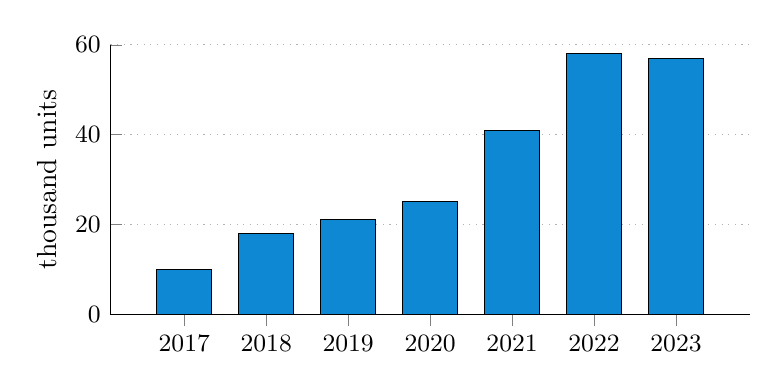
\begin{tikzpicture}
                \begin{axis}[
                        ybar,
                        bar width=20pt,
                        ymin=0, ymax=60,
                        width=0.8\linewidth,
                        height=5cm,
                        enlarge x limits=0.15,
                        axis x line*=bottom,
                        axis y line*=left,
                        ymajorgrids=true,
                        grid style={dotted,gray!60},
                        ylabel={thousand units},
                        xtick=data,
                        xticklabels={2017,2018,2019,2020,2021,2022,2023},
                        tick label style={font=\small},
                    ]
                    \addplot[fill=cyan!70!blue] coordinates {
                            (1,10)  % 2017
                            (2,18)  % 2018
                            (3,21)  % 2019
                            (4,25)  % 2020
                            (5,41)  % 2021
                            (6,58)  % 2022
                            (7,57)  % 2023
                        };
                \end{axis}
            \end{tikzpicture}
            \caption{Global annual installations of collaborative robots from 2017 to 2023 (in thousand units). Data from~\cite{Q0_3_industrial_robots_new_cobot_installations_BarChart}.}\label{fig:cobot_installations}
        \end{figure}

        The growing deployment of, and increasing collaboration with, robots imposes stringent requirements on safety and performance. 
        As tasks become more complex and humans and robots share workspaces more closely, two closely related problems become central: 
        safe manipulation of payloads and safe physical human-robot interaction. 
        Addressing both problems requires accurate knowledge of the inertial parameters of the manipulated object together with consistent estimation of the robot's dynamic state and interaction forces. 
        A collaborative robot must therefore maintain an internal representation of the mass-inertia properties of the payload or tool it manipulates and of the forces exchanged with its environment. 
        This dynamic awareness is a prerequisite for compliant, contact-rich behaviour and for precise, high-performance manipulation in close proximity to humans.
        \cite{Q1_1_fast_inertial_id_cobots, Q1_2_online_payload_mo, Q1_3_external_torque_smo, Q1_5_payload_estimation_compensation_2025, Q1_7_10947736, Q1_8_10944553, Q1_9_xu2022_double_weighting_payload_id, % chktex 2
        Q1_10_duan_payload_ftsensor, Q1_11_wei_composite_filter, Q1_13_dynamic_model_id_swevers2007, Q1_14_long2022sliding_momentum_observer, Q3_2_encoder_attention_payload}.

        \textbf{Use Case}

        The considerations above motivate a concrete use case in which a collaborative robotic arm must manipulate previously unseen objects in a shared workspace. 
        A vision system can provide geometric information such as shape and dimensions of the payload, but it does not directly reveal its mass, center of mass (CoM), or inertia tensor. 
        For safe and precise execution of contact-rich tasks, however, these inertial properties are indispensable.

        In practice, the only viable way to obtain this information during operation is to exploit the robot's own sensor data, such as joint positions, velocities and accelerations, motor currents/torques,
        and optionally wrist force/torque measurements. 
        From these signals, one can estimate both the robot's rigid-body parameters and the inertial properties of the attached payload. 
        This leads to the dual identification problem of \emph{robot dynamic parameter identification} (RDPI) and \emph{payload dynamic parameter identification} (PDPI).

        The targeted application scenario comprises typical industrial and collaborative tasks such as pick-and-place, human-assisted manipulation, and precise tool use. 
        In all these cases, RDPI and PDPI must be performed online so that the controller maintains an up-to-date model of the combined robot-payload dynamics and the resulting contact forces. 
        Robust online identification methods are therefore a key enabling technology for safe human-robot collaboration and high-performance manipulation with arbitrary payloads and tools.

    \section{Problem Description}
    The subsection \emph{Kinematic and Dynamic Background of Robot Manipulation} analyses why endowing a robotic manipulator with awareness of its own dynamics, payload, and tools is mathematically demanding and cannot be
    achieved by simple calculation or direct measurement alone. The subsection \emph{Limitations of the Current State of the Art} then identifies the main shortcomings of existing identification and estimation methods
    in the literature, thereby motivating the contribution of this work.

        \textbf{Kinematic and Dynamic Background of Robot Manipulation}
        ~\label{sec:robot_dynamics_background}
        The inertial properties of a rigid body are collected in the standard 10-dimensional parameter vector
        \begin{equation}
        \boldsymbol{\phi}^T
        =
        \begin{bmatrix}
            m & m c_x & m c_y & m c_z &
            J_{xx} & J_{xy} & J_{xz} & J_{yy} & J_{yz} & J_{zz}
        \end{bmatrix}
        \in \mathbb{R}^{10},
        \label{eq:rigidBody}
        \end{equation}
        which enters the Newton-Euler equations
        \begin{equation}
        \begin{bmatrix} 
            \mathbf{f} \\[2pt] \boldsymbol{\tau}
        \end{bmatrix}
        =
        m
        \begin{bmatrix}
            \mathbf{I}_{3\times3} & -[\mathbf{c}]^{\times} \\
            [\mathbf{c}]^{\times} & \mathbf{J}_s
        \end{bmatrix}
        \begin{bmatrix}
            \mathbf{a} \\[2pt] \boldsymbol{\alpha}
        \end{bmatrix}
        +
        \begin{bmatrix}
            m[\boldsymbol{\omega}]^{\times}[\boldsymbol{\omega}]^{\times}\mathbf{c} \\
            [\boldsymbol{\omega}]^{\times}\mathbf{J}_s\boldsymbol{\omega}
        \end{bmatrix},
        \label{eq:newtonEuler}
        \end{equation}
        so that the wrench $(\mathbf{f},\boldsymbol{\tau})$ depends nonlinearly on the motion $(\mathbf{a},\boldsymbol{\alpha},\boldsymbol{\omega})$ but linearly on $\boldsymbol{\phi}$.
        
        For the equipment rigidly attached to the tool flange (gripper/tool, with or without payload/load) we define an effective rigid-body parameter vector
        \begin{equation}
        \boldsymbol{\phi}_{\mathrm{eff}}
        =
        \begin{cases}
            \boldsymbol{\phi}_{\mathrm{tool}}, & \text{no load},\\[4pt]
            \boldsymbol{\phi}_{\mathrm{tool}} + \boldsymbol{\phi}_{\mathrm{load}}, & \text{with load},
        \end{cases}
        \label{eq:rigidEffective}
        \end{equation}
        which acts on top of the nominal robot dynamics. In contrast, with a clean flange (no tool/no load) only the robot parameters $\boldsymbol{\phi}_{\mathrm{robot}}$ contribute to the system dynamics.


        The robot structure itself is described by its own parameter vector $\boldsymbol{\phi}_{\mathrm{robot}}$, which enters the standard joint-space rigid-body dynamics. We denote this contribution by
        $\boldsymbol{\tau}_{\mathrm{robot}}$ (clean flange),
        \begin{equation}
        \boldsymbol{\tau}_{\mathrm{robot}}
        =
        \mathbf{M}(\mathbf{q}) \ddot{\mathbf{q}}
        +
        \mathbf{C}(\mathbf{q},\dot{\mathbf{q}})\dot{\mathbf{q}}
        +
        \mathbf{G}(\mathbf{q})
        +
        \boldsymbol{\tau}_f(\dot{\mathbf{q}}),
        \label{eq:robot_dynamics}
        \end{equation}
        where $\boldsymbol{\tau}_f(\dot{\mathbf{q}})$ models joint-level non-idealities such as Coulomb and viscous friction,
        possible Stribeck effects, and drive-train phenomena like backlash.
        
        The wrench generated by the effective rigid body at the flange induces an additional joint-space torque
        \begin{equation}
        \boldsymbol{\tau}_{\mathrm{ext}}
        =
        \mathbf{J}^T(\mathbf{q})\,\vec{F}_{\mathrm{ext}}(\boldsymbol{\phi}_{\mathrm{eff}}),
        \label{eq:tau_ext}
        \end{equation}
        where $\mathbf{J}(\mathbf{q})$ is the end-effector Jacobian. In the clean-flange case (no tool/no load), $\vec{F}_{\mathrm{ext}}$ reduces to purely external interaction forces with the environment (e.g.\ contacts or collisions).

    

        The motor torques are therefore
        \begin{equation}
        \boldsymbol{\tau}_{\mathrm{motor}}
        =
        \boldsymbol{\tau}_{\mathrm{robot}}
        +
        \boldsymbol{\tau}_{\mathrm{ext}}(\boldsymbol{\phi}_{\mathrm{eff}}),
        \label{eq:tau_motor}
        \end{equation}
        and for brushless DC actuators with torque constant $k_t$ one obtains the current-torque relation
        \begin{equation}
        \boldsymbol{\tau}_{\mathrm{motor}} = k_t\,\boldsymbol{I}
        \quad\Rightarrow\quad
        \boldsymbol{I}
        =
        \frac{\boldsymbol{\tau}_{\mathrm{robot}}
                + \boldsymbol{\tau}_{\mathrm{ext}}(\boldsymbol{\phi}_{\mathrm{eff}})}
            {k_t}.
        \label{eq:I_payload}
        \end{equation}

        If a force/torque sensor is mounted at the flange, the measured wrench can be written, using the relations derived in the Appendix, as
        \begin{equation}
        \vec{F}_{\mathrm{measured}}
        =
        Y\bigl(\mathbf{a},\boldsymbol{\alpha},\boldsymbol{\omega}\bigr)\,
        \boldsymbol{\phi}_{\mathrm{eff}}
        +
        \vec{F}_{\mathrm{bias}}
        +
        \vec{n},
        \label{eq:F_measured_regressor}
        \end{equation}

        where $Y(\cdot)$ is the $6\times 10$ Newton-Euler regressor matrix defined in the Appendix~\ref{app:query_categories}. It is linear in the inertial parameter vector $\boldsymbol{\phi}_{\mathrm{eff}}$, but depends nonlinearly on the motion variables $(\mathbf{a},\boldsymbol{\alpha},\boldsymbol{\omega})$. The terms $\vec{F}_{\mathrm{bias}}$ and $\vec{n}$ denote sensor bias and noise, respectively.\footnote{All experiments in this work are simulation-based; in the subsequent method formulation, sensor bias and noise are therefore neglected and \eqref{eq:F_measured_regressor} is used without $\vec{F}_{\mathrm{bias}}$ and $\vec{n}$.}
        The motion variables $(\mathbf{a},\boldsymbol{\alpha},\boldsymbol{\omega})$ are in turn determined by the joint state and motor torques through the nonlinear dynamics\eqref{eq:robot_dynamics}-\eqref{eq:I_payload}.

        From an identification viewpoint, this creates two tightly coupled challenges. 
        First, all available measurements (joint currents, positions, velocities and flange wrench) depend on the \emph{combined} dynamics of robot, tool and load via the nonlinear relationships~\eqref{eq:robot_dynamics}-\eqref{eq:F_measured_regressor}, so the contribution of the load parameters $\boldsymbol{\phi}_{\mathrm{load}}$ cannot be isolated by simple computation or direct measurement. 
        Second, accurate payload or load dynamic parameter identification (PDPI) presupposes an equally accurate compensation of the underlying robot-tool dynamics, including unmodelled effects such as friction and joint transmission nonlinearities. 
        Together, these aspects make dynamic awareness of payload, tool and robot a mathematically demanding inverse problem rather than a straightforward calculation from geometric or sensor data.